\documentclass[tikz,border=2mm]{standalone}
\usepackage{tikz}
\usetikzlibrary{positioning}

\begin{document}
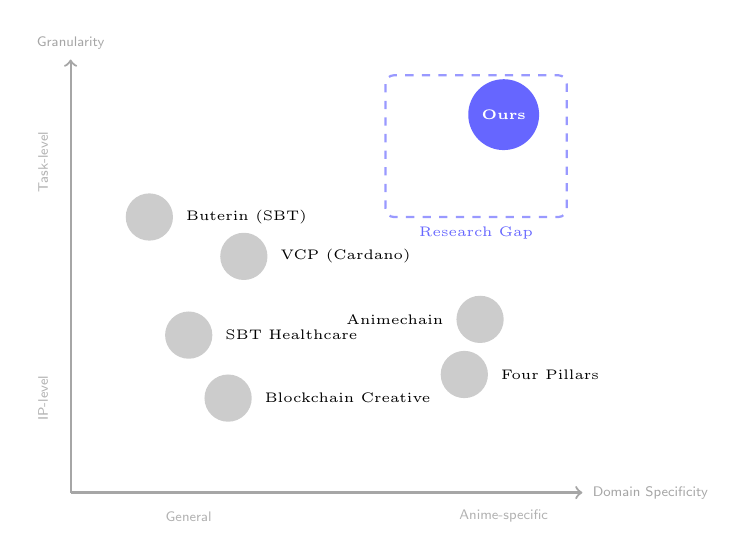
\begin{tikzpicture}[
  font=\scriptsize\sffamily
]

% Axes
\draw[->, thick, gray!70] (0,0) -- (6.5,0) node[right, font=\tiny\sffamily] {Domain Specificity};
\draw[->, thick, gray!70] (0,0) -- (0,5.5) node[above, font=\tiny\sffamily] {Granularity};

% Axis labels
\node[font=\tiny\sffamily, gray!60] at (1.5,-0.3) {General};
\node[font=\tiny\sffamily, gray!60] at (5.5,-0.3) {Anime-specific};
\node[font=\tiny\sffamily, gray!60, rotate=90] at (-0.35,1.2) {IP-level};
\node[font=\tiny\sffamily, gray!60, rotate=90] at (-0.35,4.2) {Task-level};

% Existing works (gray dots)
\node[circle, fill=gray!40, minimum size=6mm, inner sep=0pt] (v) at (1.0, 3.5) {};
\node[font=\tiny, right=1pt of v] {Buterin (SBT)};

\node[circle, fill=gray!40, minimum size=6mm, inner sep=0pt] (h) at (1.5, 2.0) {};
\node[font=\tiny, right=1pt of h] {SBT Healthcare};

\node[circle, fill=gray!40, minimum size=6mm, inner sep=0pt] (vc) at (2.2, 3.0) {};
\node[font=\tiny, right=1pt of vc] {VCP (Cardano)};

\node[circle, fill=gray!40, minimum size=6mm, inner sep=0pt] (bc) at (2.0, 1.2) {};
\node[font=\tiny, right=1pt of bc] {Blockchain Creative};

\node[circle, fill=gray!40, minimum size=6mm, inner sep=0pt] (fp) at (5.0, 1.5) {};
\node[font=\tiny, right=1pt of fp] {Four Pillars};

\node[circle, fill=gray!40, minimum size=6mm, inner sep=0pt] (ac) at (5.2, 2.2) {};
\node[font=\tiny, left=1pt of ac] {Animechain};

% AnimatorSBT (highlighted)
\node[circle, fill=blue!60, minimum size=9mm, inner sep=0pt, text=white, font=\tiny\bfseries] (ours) at (5.5, 4.8) {Ours};

% Dashed box showing the gap
\draw[dashed, thick, blue!40, rounded corners=3pt] (4.0, 3.5) rectangle (6.3, 5.3);
\node[font=\tiny, blue!60] at (5.15, 3.3) {Research Gap};

\end{tikzpicture}
\end{document}
